%%%%%%%%%%%%%%%%%%%%%%%%%%%%%%%%%%%%%%%%%
% Short Sectioned Assignment LaTeX Template Version 1.0 (5/5/12)
% This template has been downloaded from: http://www.LaTeXTemplates.com
% Original author:  Frits Wenneker (http://www.howtotex.com)
% License: CC BY-NC-SA 3.0 (http://creativecommons.org/licenses/by-nc-sa/3.0/)
%%%%%%%%%%%%%%%%%%%%%%%%%%%%%%%%%%%%%%%%%

%----------------------------------------------------------------------------------------
%	PACKAGES AND OTHER DOCUMENT CONFIGURATIONS
%----------------------------------------------------------------------------------------

\documentclass[paper=a4, fontsize=11pt]{scrartcl} % A4 paper and 11pt font size

% ---- Entrada y salida de texto -----

\usepackage{hyperref}
\usepackage{listings}
\usepackage{color}
%AÑADIDO DE LA PÁGINA http://stackoverflow.com/questions/3175105/how-to-insert-code-into-a-latex-doc
\definecolor{dkgreen}{rgb}{0,0.6,0}
\definecolor{gray}{rgb}{0.5,0.5,0.5}
\definecolor{mauve}{rgb}{0.58,0,0.82}

\lstset{frame=tb,
	language=Python,
	aboveskip=3mm,
	belowskip=3mm,
	showstringspaces=false,
	columns=flexible,
	basicstyle={\small\ttfamily},
	numbers=none,
	numberstyle=\tiny\color{gray},
	keywordstyle=\color{blue},
	commentstyle=\color{dkgreen},
	stringstyle=\color{mauve},
	breaklines=true,
	breakatwhitespace=true,
	tabsize=3
}
%%%%%%%%%%%%%%%%%%%%%%%%%%%%%%%%%%%%%%%%%%%%%%%%%%%%%%%
\usepackage{varioref}
\usepackage[T1]{fontenc} % Use 8-bit encoding that has 256 glyphs
\usepackage[utf8]{inputenc}
%\usepackage{fourier} % Use the Adobe Utopia font for the document - comment this line to return to the LaTeX default

% ---- Idioma --------

\usepackage[spanish, es-tabla]{babel} % Selecciona el español para palabras introducidas automáticamente, p.ej. "septiembre" en la fecha y especifica que se use la palabra Tabla en vez de Cuadro

% ---- Otros paquetes ----

\usepackage{amsmath,amsfonts,amsthm} % Math packages
%\usepackage{graphics,graphicx, floatrow} %para incluir imágenes y notas en las imágenes
\usepackage{graphics,graphicx, float} %para incluir imágenes y colocarlas

% Para hacer tablas comlejas
%\usepackage{multirow}
%\usepackage{threeparttable}

%\usepackage{sectsty} % Allows customizing section commands
%\allsectionsfont{\centering \normalfont\scshape} % Make all sections centered, the default font and small caps

\usepackage{fancyhdr} % Custom headers and footers
\pagestyle{fancyplain} % Makes all pages in the document conform to the custom headers and footers
\fancyhead{} % No page header - if you want one, create it in the same way as the footers below
\fancyfoot[L]{} % Empty left footer
\fancyfoot[C]{} % Empty center footer
\fancyfoot[R]{\thepage} % Page numbering for right footer
\renewcommand{\headrulewidth}{0pt} % Remove header underlines
\renewcommand{\footrulewidth}{0pt} % Remove footer underlines
\setlength{\headheight}{13.6pt} % Customize the height of the header

\numberwithin{equation}{section} % Number equations within sections (i.e. 1.1, 1.2, 2.1, 2.2 instead of 1, 2, 3, 4)
\numberwithin{figure}{section} % Number figures within sections (i.e. 1.1, 1.2, 2.1, 2.2 instead of 1, 2, 3, 4)
\numberwithin{table}{section} % Number tables within sections (i.e. 1.1, 1.2, 2.1, 2.2 instead of 1, 2, 3, 4)

\setlength\parindent{0pt} % Removes all indentation from paragraphs - comment this line for an assignment with lots of text

\newcommand{\horrule}[1]{\rule{\linewidth}{#1}} % Create horizontal rule command with 1 argument of height


\renewcommand{\reftextbefore}
	{en la  \reftextvario{página que precede a esta}{página anterior}}
\renewcommand{\reftextafter}
	{en la \reftextvario{siguiente}{siguiente} página}
\renewcommand{\reftextfacebefore}
	{en la  \reftextvario{anterior}{anterior} página}
\renewcommand{\reftextfaceafter}
	{en la \reftextvario{siguiente}{siguiente}{página}}

 \usepackage{algpseudocode}
%----------------------------------------------------------------------------------------
%	TÍTULO Y DATOS DEL ALUMNO
%----------------------------------------------------------------------------------------

\title{	
\normalfont \normalsize 
\textsc{{\bf Algorítmica (2015-2016)} \\ Grado en Ingeniería Informática \\ Universidad de Granada} \\ [25pt] % Your university, school and/or department name(s)
\horrule{0.5pt} \\[0.4cm] % Thin top horizontal rule
\huge Práctica 3- Segunda Parte: Travel Salesman Problem \\ % The assignment title
\horrule{2pt} \\[0.5cm] % Thick bottom horizontal rule
}

\author{Francisco Carrillo Pérez,Borja Cañavate Bordons, \\Miguel Porcel Jiménez,Jose Manuel Rejón Santiago,Jose Arcos Aneas} % Nombre y apellidos

\date{\normalsize\today} % Incluye la fecha actual

%----------------------------------------------------------------------------------------
% DOCUMENTO
%----------------------------------------------------------------------------------------

\begin{document}

\maketitle % Muestra el Título

\newpage %inserta un salto de página

\tableofcontents % para generar el índice de contenidos

\listoffigures

\listoftables

\newpage


	\section{Introducción }
	
		\begin{itemize}
			\item El objetivo de esta práctica es diseñar varios algoritmos Greedy resolviendo el problema del viajante de comercio o TSP
		\end{itemize}
	
	
	
	%------------------------------------------------
	\section{Primera versión} 


		Aplicar algoritmo usando Greedy simple, buscaremos en cada momento la ciudad más cercana y esa ciudad
		la añadiremos a nuestro conjunto de soluciones. 
		
	
	
	%------------------------------------------------
	\subsection{Diseño del algoritmo} 
	
			\begin{itemize}
			\item \textbf{Conjunto de candidatos}: Conjunto de ciudades. (Conjunto \textbf{C})
			\item \textbf{Conjunto de seleccionados}: Conjunto de ciudades ordenado. (Conjunto \textbf{S})
			\item \textbf{Función solución}: Cuando el conjunto de candidatos esté vacío.
			\item \textbf{Función factibilidad:} Cuando la ciudad no ha sido visitada.
			\item \textbf{Función selección}: Se seleccionará la ciudad más cercana.
			\item \textbf{Función objetivo}: Lista con las ciudades en el orden en el que hay que visitarlas.		
		\end{itemize}		
		
	\subsection{Pseudocodigo}
	
		
		\begin{algorithmic}
			\Require Conjunto de ciudades C,S
			\State {x=0}
			\State {S=C[0]}
			\For {i = 1 to len(C)}
			\If{ C[i] MenorDistancia }
			\State{x = C[i]}
			\State{S.add(x)}
			\State{C[i].erase}
			\EndIf
			\EndFor  
			
			\Return S	
		\end{algorithmic}	
	
	
	
	%------------------------------------------------
	\section{Segunda versión} 
	
		Aplicar algoritmo usando Greedy con selección parcial, estableceremos un recorrido inicial seleccionando las 3 ciudades más alejadas (oeste, norte y este). A partir de ahí añadiremos las ciudades con respecto a los intervalos creados.
		

	
	%------------------------------------------------
	\subsection{Diseño del algoritmo} 
	
		\begin{itemize}
			\item \textbf{Conjunto de candidatos}: Conjunto de ciudades. (Conjunto \textbf{C})
			\item \textbf{Conjunto de seleccionados}: Conjunto de ciudades ordenado. (Conjunto \textbf{S})
			\item \textbf{Función solución}: Cuando el conjunto de candidatos esté vacío.
			\item \textbf{Función factibilidad:} Cuando la ciudad no ha sido visitada.
			\item \textbf{Función selección}: Se seleccionará una ciudad y comprobaremos para cada una de las posiciones del circuito solución el mejor lugar para insertarlo (la que ofrece menor distancia) .
			\item \textbf{Función objetivo}: Lista con las ciudades en el orden en el que hay que visitarlas.		
		\end{itemize}
		
	
	
	\subsection{Pseudocódigo}
			
		
		\begin{algorithmic}				
			\Require Conjunto de ciudades C,S
			\State {x=0; S=CalcularRecorridoInicial();}
			\While {C}
				\For {i=0 to len(C)}
					\State{x = C[i];}
					\For{ j=1 to len(S-1)}
						\State {Saux = S; Saux[j] = x;}
						\If {distanciaSaux menor que minDistancia}
							\State {minDistancia = distanciaSaux;}
							\State {indiceSolucion = j; indiceCiudad = i;}
						\EndIf
					\EndFor
				\EndFor 
				\State{S[indiceSolucion] = x; C[indiceCiudad].erase;}
			\EndWhile 
			
			\Return S
		
		\end{algorithmic}

	
	\section{Tercera versión} 
	
		Implementación del algoritmo Greedy 2-Opt. Calcularemos una primera aproximación de la solución utilizando el algoritmo de la primera versión. Después, iremos para cada ciudad intercambiando con las siguientes, viendo si alguno de esos intercambios mejora la primera solución obtenida, así hasta intentar generar una solución mejor que la primera
		
	%------------------------------------------------
	\subsection{Diseño del algoritmo} 
	
		\begin{itemize}
			\item \textbf{Conjunto de candidatos}: Conjunto de ciudades. (Conjunto \textbf{C})
			\item \textbf{Conjunto de seleccionados}: Conjunto de ciudades ordenado. (Conjunto \textbf{S})
			\item \textbf{Función solución}: Cuando el conjunto de candidatos esté vacío.
			\item \textbf{Función factibilidad:} Cuando la ciudad no ha sido visitada.
			\item \textbf{Función selección}: Dada la solución con la primera versión del algoritmo, comprobaremos si intercambiando una por una las ciudades se mejora la solución inicial.
			\item \textbf{Función objetivo}: Lista con las ciudades en el orden en el que hay que visitarlas.		
		\end{itemize}
		
		
	\subsection{Pseudocódigo}

		\begin{algorithmic}				
			\Require Conjunto de ciudades C,S,AUX
			\State S=PrimeraVersión();Z=Distancia(S);
			\State {x,y,i = 0; j = 1;}
			\While {\textbf{i} menor o igual \textbf{tam -2} and\textbf{ j} menor o igual a \textbf{tam - 1}}
			\State Sp=Swap(S,i,j);Zp=Distancia(Sp);
			\If {\textbf{Zp} mayor o igual que \textbf{z} and \textbf{j} menor que \textbf{tam-1}}
			\State j++;
			\EndIf
			\If{\textbf{zp} mayor o igual que \textbf{z} and \textbf{j }== \textbf{tam - 1}}
			\State j += 1; i += 1
			\EndIf
			\If {\textbf{zp }menor que \textbf{z}}
			\State S = Sp; Z = Zp;
			\State i += i; j = i + 1;
			\EndIf
			\EndWhile  
			
			\Return S	
			
			
			
		\end{algorithmic}
		

	\section{Comparación}

		En esta sección veremos los distintos resultados obtenidos de cada una de las ejecuciones de los algoritmos.
		
		\begin{table}[H]
			\centering
			
			
			\begin{tabular}{l|l|l|l|l}
				Mapa & Versión I & Versión II & Versión III  & Versión óptima  \\
				ulysses16 & 79.0141 & 81.1402 & 74.4295 & - \\
				berlin52 & 8314.81 & 9622.17 & 7883.92 & 7542  \\
				ch130 & 7022.12 & 7499.39 & 6738.84 & 6110 \\
				lin105 & 17173.4 & 19159.3 & 16139.2 & 14379 \\
				kroa100	& 25345.7 & 27646.1 & 24163.5 & 21282 \\
				pcb442 & 61536.8 & 61217.7 & 59520.4 & 50778 \\
			\end{tabular}
			
		\end{table}
		

		En esta sección veremos los distintos grafos obtenidos de cada uno de los algoritmos para el mapa Berlin52
		
		\begin{figure}
			\centering
			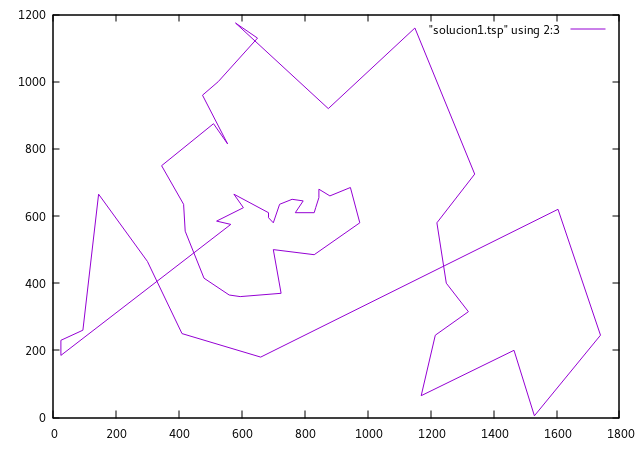
\includegraphics[width=0.7\linewidth]{../grafica/grafica1.png}
			\caption{Primera versión}
			\label{fig:graficafinal}
		\end{figure}
		

		En esta sección veremos los distintos grafos obtenidos de cada uno de los algoritmos para el mapa Berlin52
		
		\begin{figure}
			\centering
			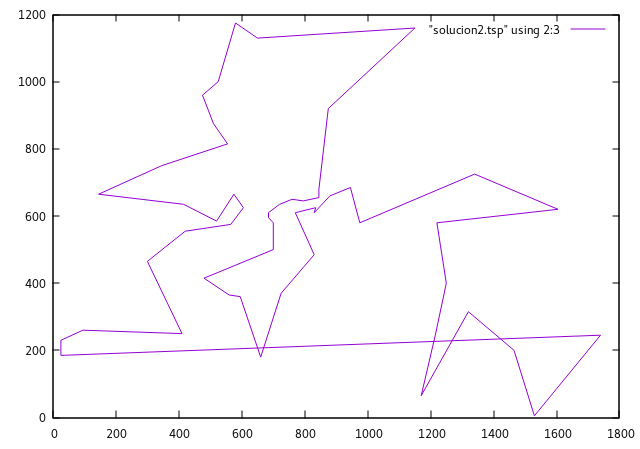
\includegraphics[width=0.7\linewidth]{../grafica/grafica2.png}
			\caption{Segunda versión}
			\label{fig:graficafinal}
		\end{figure}
		
		
		

		En esta sección veremos los distintos grafos obtenidos de cada uno de los algoritmos para el mapa Berlin52
		
		\begin{figure}
			\centering
			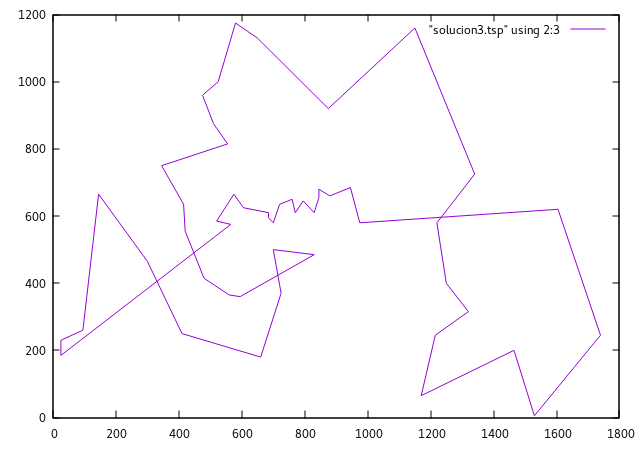
\includegraphics[width=0.7\linewidth]{../grafica/grafica3.png}
			\caption{Tercera versión}
			\label{fig:graficafinal}
		\end{figure}
		
		
	
	
	
	
\end{document} 